% Created 2021-12-17 Fri 17:10
\documentclass[9pt, b5paper]{article}
\usepackage[UTF8]{ctex}
\usepackage{xltxtra}
\usepackage{bera}
\usepackage[T1]{fontenc}
\usepackage[scaled]{beraserif}
\usepackage[scaled]{berasans}
\usepackage[scaled]{beramono}
\usepackage{graphicx}
\usepackage{xcolor}
\usepackage{multirow}
\usepackage{multicol}
\usepackage{float}
\usepackage{textcomp}
\usepackage{geometry}
\geometry{left=1.2cm,right=1.2cm,top=1.5cm,bottom=1.2cm}
\usepackage{algorithm}
\usepackage{algorithmic}
\usepackage{latexsym}
\usepackage{natbib}
\usepackage{minted}
\newminted{common-lisp}{fontsize=ootnotesize}
\usepackage[xetex,colorlinks=true,CJKbookmarks=true,linkcolor=blue,urlcolor=blue,menucolor=blue]{hyperref}
\author{deepwaterooo}
\date{\today}
\title{Android Study Plan}
\hypersetup{
  pdfkeywords={},
  pdfsubject={},
  pdfcreator={Emacs 27.1 (Org mode 8.2.7c)}}
\begin{document}

\maketitle
\tableofcontents


\section{Daily updates}
\label{sec-1}
\begin{itemize}
\item 因为需要准备一个面试,这几天不更新算法系列,只准备安卓面试
\item win 10 wsl 1 ubuntu 18 adb configuration done, not complicated, once search for solutions, and config, it works.
\item api levle 30 androidx basic project environment can be configured, but dynamic fragment add not done yet, switched back to api 28 temporatorily
\item wsl 1 ubuntu 18 adb logcat is so slow. after 9pm yesterday, 150K lines of log, I could only adb logcat previous project samplefragments, can can not grab any FirstFragment nor Second Fragment Log.i info. may switch laptop back to Mac, but it has only 8GB memory, and internet too slow for that laptop
\item today will review major components, as well small details, notes summaries to move on
\item \textbf{恶鬼们昨天晚上今天早上又疯狂作案一晚,一个故意晚回来,用洗手间,用厨房,半夜一两点钟还在故意厨房里开厨导柜吵别人;一个今天早上五点钟便受恶房东暗示指使,故意开车库噪音极大的声响,早上五点钟便故意吵醒别人休息,实在是无恶不作(它有昨天晚上下班后到休息前一晚上的时间他不提前装车,非要等到早上五点钟故意把别人吵醒,另一个贱畜牲的做法是在别人晚上入睡前故意吵别人,贱蓄牲们的做法还不够猖狂吗?)}
\item BroadcastReceiver sample project runs though easily. Will look into ContentProvider projects too today, all of them are not complicated.
\item ContentProvider Interprocess communication projects are connected well too. One functions as server, the other as client, not complicated at all.
\item The coding interview is done (due to the interface reasons, the 120 minutes test was submitted in about 60 minutes by mistake, the coding test interface does not false-positive submit proof), expecting the final round of interview, while at the same time, I am returning back to algorithms, and tomorrow there is a weekly contest too.
\end{itemize}

\section{职场弱弱的奔溃瞬间(+1)}
\label{sec-2}
\begin{itemize}
\item 联系我安排面试相关的按照名字来看,应该是一个美国人吧,关于文化、语言等,这样的hr写邮件与candidate沟通应该会相对比较顺利一点
\end{itemize}

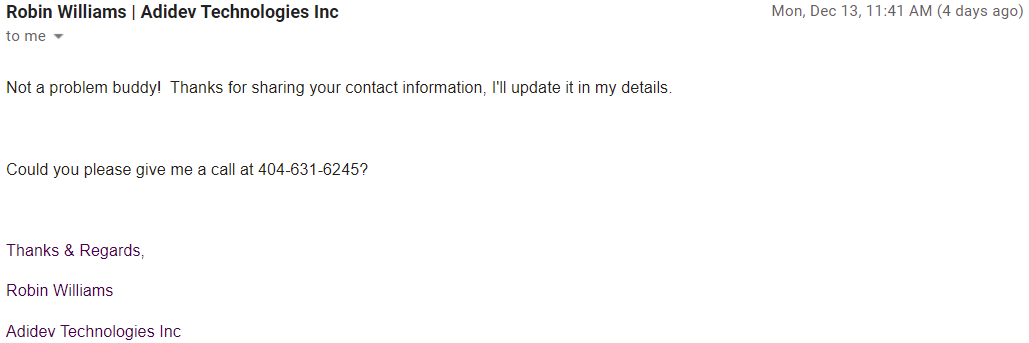
\includegraphics[width=.9\linewidth]{./pic/buddy.png}
\begin{itemize}
\item 偶这个职场弱弱,瞬间被这五个字母吓傻了,怎么也不敢跟他们联系,直到下午约定的时候中介打电话进来。
\item 记得上次与另一个公司的第一轮面试快结束时问及第二轮的coding test是怎么样的,会是像leetcode之类的刷题界面一样吗?我是一个emacs依赖症重症患者,离开command line based editor emacs,我不会写代码。记得当时与面试官沟通这个问题的时候,他说到会sharing screen, 这个我们面试者就可以在自己最熟悉与舒适的工作环境中尽可能高效地答题、写出理想的代码。
\item 今天早上,当我第一时间读及收件箱邮件里的reminder, 

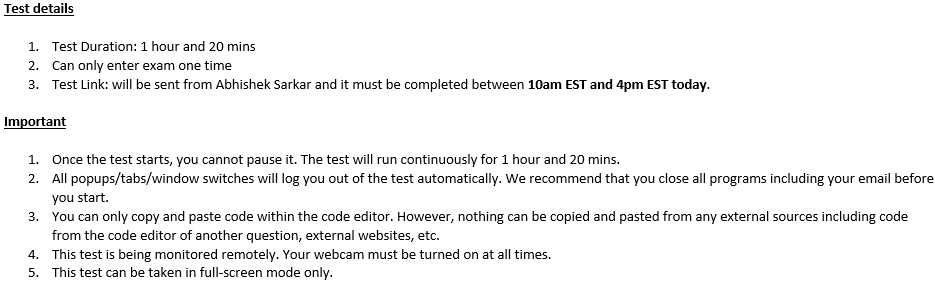
\includegraphics[width=.9\linewidth]{./pic/req.png}
\begin{itemize}
\item 作为一个久经沙场、久经面试的弱弱,内心瞬间奔溃、溃不成军。。。。。。这究竟是要干什么???
\item 好在,作为一个久经沙场,久经面试的弱弱,死猪不怕开水烫,大不了就是不是command line based editor的界面会写得慢、会写得不顺,会无数次敲错字符,会写出来的代码不成型,bug多,极度降低效率,但它好歹还是一个test不是?这种test的机会也不是很多呀
\item 于是,偶们还是硬着头皮明知山有虎地跑去把coding test给做了。。。
\end{itemize}
\item 回想2012年9月还是10月继自己装linux系统把电脑弄坏之后,被自己作业c++代码里的一个bug吓得魂飞魄散,急忙给代课教师写邮件求救。。。。。。原来这么多年过去了,偶们还是这么一个弱弱。。。。。。
\end{itemize}

\section{系统服务篇}
\label{sec-3}
:clock1: DONE: Android 如何启动?
[x] DONE: Android 应用进程启动流程
[ ] 什么是系统服务?
[ ] ActivityManagerService
[ ] SystemServer
[x] DONE: Android 应用安装过程源码解析
[ ] WindowManagerService
[ ] Zoyote 前世今生

\section{通信框架篇}
\label{sec-4}
[x] Binder 完全解析
[x] DONE: Binder 完全解析(一)概述
[x] DONE: Binder 完全解析(二)设计详解
[x] DONE: Binder 完全解析(三)AIDL实现原理分析
[x] Handler 通信框架
[x] DONE: Handler消息机制源码解析

\section{应用组件篇}
\label{sec-5}
[ ] Application 是什么?
DONE: Context 分析
[ ] Activity 组件分析
[x] DONE: Activity生命周期是如何实现的
[ ] Services 组件分析
[ ] ContentProvider 组件分析
[ ] Broadcast 组件分析

\section{珠玑拾遗}
\label{sec-6}
[ ] Gradle 用法
[ ] 混淆一二事

Andriod系统开发

\section{Android操作系统概述}
\label{sec-7}
Android平台介绍;Android平台特性;Android平台架构;Android Navtive C/C++程序开发;Android NDK;Native开发方式与JAVA开发方式比较。
\section{Android开发环境搭建}
\label{sec-8}
Android SDK介绍;Eclipse ADT插件;Android模拟器开发。
\section{Android项目结构分析}
\label{sec-9}
资源管理(Resources)分析;drawable分析;layout分析;Activity分析;Intent分析;Service分析;Content分析。
\section{Android UI设计}
\label{sec-10}
标准控件的使用;设计开发自定义控件;Layout布局的使用;触摸/按键(UI Events)事件处理方法;View,SurfaceView,Canvas,Paint类分析使用;显示文本以及显示特殊效果文本;绘图及显示图片;实现动画效果。
\section{Intent Receive}
\label{sec-11}
Intent的作用和目的;属性讲解;Android定义解析Intent;AndroidManifest.xml深入分析。
\section{Service}
\label{sec-12}
什么是Service,如何使用Service,Service的生命周期,BroadcastReceiver的使用。
\section{Content Provider}
\label{sec-13}
SQLite介绍,创建Content Providers,使用Content Providers,使用URI语法进行增删改查。
\section{Android高级应用开发}
\label{sec-14}
访问本地通讯录;网络连接的相关知识;流媒体的处理;URLConnection和HttpURLConnection的应用;
HttpClient的分析;本地文件浏览管理;音视频播放处理;Widget应用开发。
\section{Android程序发布部署建}
\label{sec-15}
Android 调试桥;启用logcat日志调试;模拟器上安装删除软件;打包* 签名和安装软件到设备。
\section{Android 底层架构分析}
\label{sec-16}
移植Android到新的硬件平台;需要支持Linux 操作系统的硬件平台架构分析;支持Android的Linux内核特性分析;为Linux内核增加Android特性;移植Android Debug Bridge调试接口;编写/移植Android内核驱动;硬件支持double frame buffer/page flipping;bionic库移植与优化;Dalvik Vm移植;第三方应用程序移植;建立Android移植开发平台;新的嵌入式处理器引入的Android相关问题;获得高效的Android工具链。
\section{Android移植}
\label{sec-17}
支持ARM11的Linux-2.6.28内核新特性简介;移植LCD double buffer驱动;移植触摸屏驱动;移植Android键盘驱动;移植Wifi驱动支持Android上网功能;移植电源管理驱动,支持Android电池管理;部署Android系统到实际ARM11平台。
\section{阶段项目实战与测试}
\label{sec-18}
通过对ITelephony接口和ISms接口以及AIDL在Android程序中的开发应用,开发一个打电话和发短信的程序。

\section{自定义view Android 11 api level android M}
\label{sec-19}
\subsection{gradle.properties}
\label{sec-19-1}
\begin{minted}[frame=lines,fontsize=\scriptsize,linenos=false]{xm}
android.useAndroidX=true
landroid.enableJetifier=true
\end{minted}
\begin{itemize}
\item 什么是Jetifier? 例如,要使用androidx打包的依赖项创建新项目,此新项目需要在gradle.properties文件中添加以下行:
\end{itemize}

java version 8
 compileOptions \{
        sourceCompatibility JavaVersion.VERSION$_{\text{1}}$$_{\text{8}}$
        targetCompatibility JavaVersion.VERSION$_{\text{1}}$$_{\text{8}}$
    \}

import android.os.Bundle;
import android.support.design.widget.FloatingActionButton;
import android.support.design.widget.Snackbar;
import android.view.View;
import android.view.Menu;
import android.view.MenuItem;
import androidx.appcompat.app.AppCompatActivity;
import androidx.appcompat.widget.Toolbar;
import com.google.android.material.floatingactionbutton.FloatingActionButton;
import com.google.android.material.snackbar.Snackbar;

<com.me.generalprac.CustomTitleView
    android:layout$_{\text{width}}$="match$_{\text{parent}}$"
    android:layout$_{\text{height}}$="wrap$_{\text{content}}$"/>
<include layout="@layout/custom$_{\text{title}}$"/>
% Emacs 27.1 (Org mode 8.2.7c)
\end{document}